\subsection{Enfoque al usuario}
Una gran parte del objetivo marcado en el apartado 3.1 Diseno, viene definido por el servicio que queramos ofrecerle
al usuario, ya que este, es nuestro cliente final y al que pretendermos ayudar.\\


Deberemos ser conscientes de necesidades que muestran los usuarios en combinacion con las carencias del mercado ya que
nos ayudara a saber cual puede ser la demanda o el hueco que aun no esta cubierto.
Tanto si nuestro publico objetivo, es unico, es decir tomar todos los tipos de usuarios por igual, considerando el 
usuario medio, como para un usuario caracteristico, deberemos saber las caracteristicas homogeneas de nuestro grupo.

Por lo tanto necesitamos un estudio actual sobre el nivel psicologico, social y economico del grupo objetivo, para descubrir, no solo
las necesidades, pero tambien los deseos, que le gustaria tener y sus demandas, que quieren.

Una vez los usuarios tengan acceso a los datos tal y como se los proporcionamos, es importante tener una retroalimentacion, 
seria ideal poder realizar un analisis del comportamiento del usuario para ve sus pautas respecto a los datos obtenidos.

\subsubsection{How to solve it} 
Definir a que tipo de usuarios va dirigido. Estudiar tanto sus caracteristicas como la situacion del
mercado.
Utilizar un mecanismo que nos ayude a obtener una retroalimentacion, ya sea por un sistema de puntualizaciones, test o
un mecanismo automatico que permita conocer el comportamiento del usuario. Tambien podremos optar por la combinacion de ambas 
opciones.

\subsubsection{How we solve it. Aire Guru} 
Aire Guru va dirigido a toda la poblacion, por lo que tendremos en cuenta a la hora de implementarlo que la informacion debe
mostrarse de una forma simple, ademas de completa. Ademas, ponemos especial atencion a los usuarios que puedan tener una
enfermedad o condicion medica influenciada por la polucion del aire.
Durante el estudio de mercado, nos dimos cuenta, que muchas de ellas ofrecian la polucion del aire a tiempo real, pero 
pudimos ver las siguientes carencias:
\begin{itemize}
    \item Obsolete measurements. Measurements need to be taken regularly, since there can be huge differences
    between pollution levels at different times of the day.
    \item Limited geographic coverage. The data must cover a reasonable proportion of areas that people spend significant time in.
    \item Insufficiently granular measurements. Measurements must be at a reasonably fine level of granularity. One single measurement for an entire city is not useful.
    \item Poor presentation. Often the information is presented in an uninterpreted form, making it difficult for users to visualize, especially in a geographic sense.
    \item Poor discrimination and interpretation. Many tools show individual values as a number or a colour. This information is not
    enough for the user to take control of their exposure. Such visualizations are not really compelling. 
    \item Exposicion a la polucion de una forma personalizada. Nos interesa saber a que nivel de polucion estamos expuesto
    a lo largo del tiempo, no de forma puntual.
    \item Necesidad de utilizar complicated devices para monitorizar la exposicion. Nuestro objetivo es facilitar la informacion a los 
    usuarios con el minimo de complicaciones posibles.
    \item Sin informacion dedicada por condicion medica. 
\end{itemize}

Una vez implementado, probamos la herramienta con 14 usuarios. Nuestra herramienta integra Google Analytis que nos permite saber el 
comportamiento de los usuarios, como a cuantas paginas acceden, a cuales y cuanto tiempo permanencen en ella. Ademas, finalizada la prueba,
se realizo una encuesta para medir no solo el nivel de satisfaccion, pero tambien para comprobar la utilidad y si habia conseguido el objetivo.
\begin{figure}[ht]
    \centering
   \subfigure[Aire Guru Form]
    {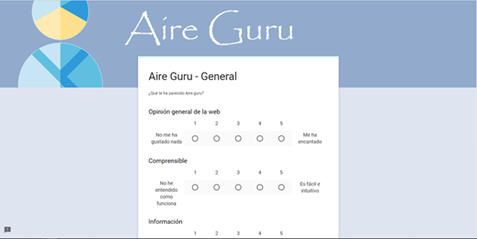
\includegraphics[width=5.5cm  ]{form}}
    \hfill
    \subfigure [Google Analytics]
       { 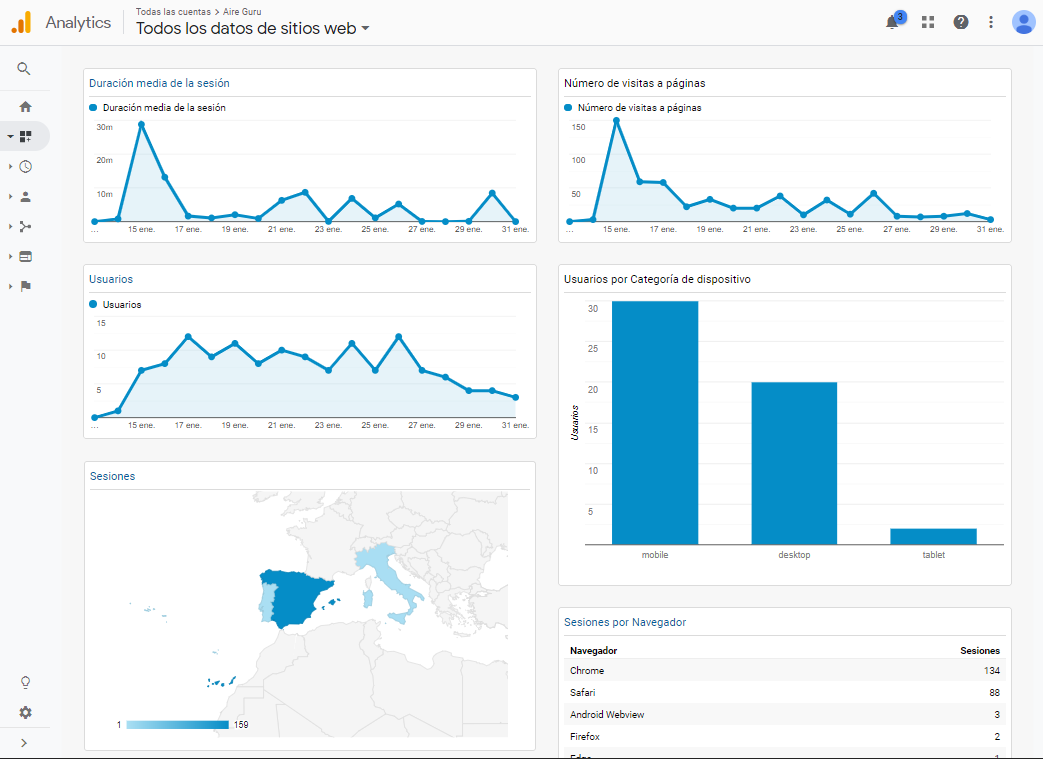
\includegraphics[width=5.5cm]{googleAnalytics}}
  
  \caption{User Feedback}
    \end{figure}
 
\elsparagraph{Evaluation}  
\begin{itemize}
    \done El estudio de mercado nos hizo ver con claridad las carencias que existen en las aplicaciones actuales.
    \done La encuesta nos reporto valoraciones muy positivas respecto a la utilizacion, comprension e informacion reportada.
    \done Usuarios nos comentaron que gracias a Aire Guru habian descubierto que tenian una condicion medica que se puede ver afectada por
    la polucion del aire

\end{itemize}
 

\newpage